\chapter{Evaluation der Ergebnisse}\label{evaluation}

Im Folgenden werden die entwickelten Modelle untersucht und evaluiert. Für die beiden \acl{RF}-Modelle wird die Implementierung von \texttt{sklearn} genutzt, für die Gradient Boosted Trees die Bibliothek \texttt{XGBoost}, da das dort verwendete \acl{XGB} besser ist als die Implementierung in \texttt{sklearn}.\footcite[Kapitel 10]{Harrison2019} Die Ergebnisse der Modelle werden sowohl für das reduzierte als auch das vollständige Merkmalsset berechnet, verglichen und aufbauend darauf die Merkmalsauswahl optimiert. Außerdem wird der Einfluss der gewählten Segmentlänge und des gewählten Schwellwertes der Annotation untersucht. Für alle Untersuchungen wird das gleiche Testset wie in Kapitel \ref{analyse} verwendet.

\section{Modellevaluation} %TODO: besserer Titel? Merkmalsauswahl?

Zunächst werden alle Modelle sowohl mit dem vollständigen Merkmalsset als auch dem reduzierten Merkmalsset verglichen; die Ergebnisse sind inTabelle \ref{fig:comparison-all} gezeigt. Insgesamt zeigt sich bereits, dass eine deutlich höhere Coverage als bei der reinen Betrachtung der Intervallschätzer des CLIE-Algorithmus erreicht wird. Diese lag beispielsweise für $q\textsubscript{th} = 0.3$ bei 20,93\,\% mit einem \ac{MAE} von 13,90\,\si{FE}. Die Ergebnisse der Klassifikation mit Gradient Boosted Trees und \acl{RF}s sind zunächst ähnlich. Bei der Regression erreichen Gradient Boosted Trees eine sehr hohe Coverage von über 80\,\% mit einem zu den anderen Modellen verhältnismäßig hohen \ac{MAE} von über 16\,\si{FE}.

	\begin{table}[H]
	\centering
		\begin{tabular}{l | l | l|| c | c | c | c }
 						& Merkmalsset	& Modell			& \ac{MAE} [FE]	& Coverage [\%]	& F1-Score	& AUC	\\ \hline
 		\multicolumn{3}{l ||}{insgesamt}					& 21{,}85		& -				& - 		& -		\\
 		\multicolumn{3}{l ||}{annotiert}					& 3{,}28			& 43{,}21		& - 		& -		\\ \hline
 		\multirow{4}{*}{Klassifikation}
 						& \multirow{2}{*}{reduziert}		
 										& \acs{RF} 		& 13{,}87		& 32{,}09		& 0{,}54	& 0,69	\\
 						&				& \acs{XGB}		& 13,14			& 29,79			& 0{,}53	& 0,69	\\\cline{2-7}
 						& \multirow{2}{*}{alle}
 									 	& \acs{RF}		& 12{,}11		& 36,81			& 0{,}61	& 0,75	\\
 						&				& \acs{XGB} 	& 11,38			& 35,93			& 0,62		& 0,75\\\hline
 		\multirow{4}{*}{Regression}
 						& \multirow{2}{*}{reduziert}
 										& \acs{RF}		& 14,34			& 41,21			& 0,57		& 0,69	\\
 						&				& \acs{XGB}		& 17,79			& 80,77			& 0,63		& 0,69	\\\cline{2-7}
 					 	& \multirow{2}{*}{alle}		
 					 					& \acs{RF}		& 12,56			& 46,27			& 0,64		& 0,75\\
 					 	&				& \acs{XGB} 		& 16,04			& 81,80			& 0,65		& 0,74\\
		\end{tabular}
		\caption{Vergleich der aller Modelle mit reduziertem und vollständigem Merkmalsset}
		\label{fig:comparison-all}
	\end{table}

Des Weiteren zeigt sich, dass das reduzierte Merkmalsset entgegen der Erwartungen zu etwas schlechteren Ergebnissen führt. Eine Betrachtung der Wichtigkeit der Merkmale für die Modelle mit vollständigem Merkmalsset zeigt, dass hier jeweils $\text{ratio}\textsubscript{acf}$ und $\text{ratio}\textsubscript{acf}$ zu den wichtigsten Merkmalen gehören, welche beide kein Teil des reduzierten Merkmalssets. In Abbildung \ref{fig:rf-clf-all-importances} ist die Verteilung der Relevanz der Merkmale gezeigt. Ein Test mit einem \ac{RF}-Klassifikator mit dem reduzierten Merkmalsset zuzüglich den oben genannten Merkmalen zeigt, dass die Performance im Vergleich zum vollständigen Merkmalsset so vergleichbar ist und ein \ac{MAE} von 11,97\,\si{FE} bei einer Coverage von 36,51\,\% erreicht wird.

\begin{figure}[H]
	\centering
	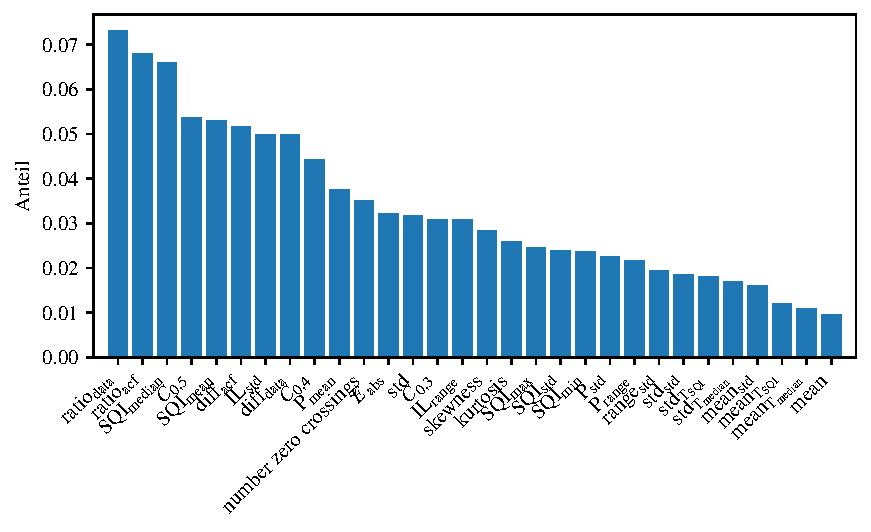
\includegraphics{pic/rf-clf-all-importances.pdf}
 	\caption{Wichtigkeit der Merkmale des \ac{RF}-Klassifikators mit vollständigem Merkmalsset}
 	\label{fig:rf-clf-all-importances}
\end{figure}

Bei den folgenden Untersuchungen wird aus diesem Grund das erweiterte reduzierte Merkmalsset verwendet. Die Ergebnisse der vier Modelle sind in Tabelle \ref{fig:final-results-comparison} abgebildet. Alle erzielen ähnliche Ergebnisse, wobei die Regressionsmodelle eine etwas höhere Coverage erreichen. Es gibt im Gegensatz zu den vorherigen Ergebnissen keine Ausreißer. Die \ac{AUC} zeigt, dass alle Modelle bei den gegebenen Daten in der Lage sind, informatives und nicht informatives Signal zu separieren.
%\begin{multicols}{2}
%\begin{itemize}
%	\item Mittelwert
%	\item Kurtosis
%	\item Schiefe
%	\item $\text{diff}\textsubscript{acf}$
%	\item $\text{diff}\textsubscript{data}$
%	\item $\text{ratio}\textsubscript{acf}$
%	\item $\text{ratio}\textsubscript{data}$
%	\item $\text{SQI}\textsubscript{std}$
%	\item $\text{SQI}\textsubscript{min}$
%	\item $\text{SQI}\textsubscript{median}$
%	\item $\text{P}\textsubscript{range}$
%	\item $\text{P}\textsubscript{mean}$
%	\item $\text{mean}\textsubscript{T\textsubscript{median}}$
%	\item $\text{std}\textsubscript{T\textsubscript{median}}$
%	\item $\text{mean}\textsubscript{T\textsubscript{SQI}}$
%	\item $\text{std}\textsubscript{T\textsubscript{SQI}}$
%	\item $\text{IL}\textsubscript{std}$
%	\item $\text{mean}\textsubscript{std}$
%	\item $C_{0,5}$
%	\item $C_{0,4}$
%	\item $C_{0,3}$
%\end{itemize}
%\end{multicols}

\begin{table}[H]
	\centering
	\begin{tabular}{l | l || c | c | c | c }
									& Modell			& \ac{MAE} [FE]	& Coverage [\%]	& F1-Score	& AUC	\\ \hline
 	\multicolumn{2}{l ||}{insgesamt}					& 21{,}85		& -				& - 		& -		\\
 	\multicolumn{2}{l ||}{annotiert}					& 3{,}28			& 43{,}21		& - 		& -		\\ \hline
 	\multirow{2}{*}{Klassifikation}
 									& \acs{RF} 		& 11,86			& 34,90			& 0,60		& 0,75	\\
 									& \acs{XGB}		& 12,44			& 41,99			& 0,63		& 0,75	\\\hline 
 	\multirow{2}{*}{Regression}
 									& \acs{RF}		& 12,57 			& 46,36			& 0,64		& 0,75	\\
 									& \acs{XGB}		& 12,66			& 47,59			& 0,64		& 0,74	\\\hline
 	\end{tabular}	
	\caption{Vergleich der aller Modelle mit finalem Merkmalsset}
	\label{fig:final-results-comparison}
\end{table}

	
Betrachtet man die Wichtigkeit der Merkmale der beiden Klassifikationsmodelle, fällt auf, dass bei dem \ac{XGB}-Klassifikator ein Merkmal allein deutlich wichtiger als alle anderen ist; sowohl beim reduzierten als auch beim vollständigen Merkmalsset. Bei den \ac{RF}-Modellen dagegen ist die Wichtigkeit gleichmäßiger verteilt. Der direkte Vergleich ist in Abbildung \ref{fig:importances-comparison-rf-xgb-clf} zu sehen. Trotz der unterschiedlichen Gewichtung der Merkmale erzielen beide Modelle ähnliche Ergebnisse. Allerdings ist der \ac{XGB}-Klassifikator weniger stabil für Verzerrung in dem mit Abstand wichtigstem Merkmal $C_{0{,}5}$. Es zeigt aber auch, dass die Ähnlichkeit der Intervallschätzer des \ac{CLIE}-Algorithmus ein gutes Kriterium zur Beurteilung der Signalqualität ist.

 \begin{figure}[h]
 	\centering
		\begin{subfigure}{.49\textwidth}
			\centering
 			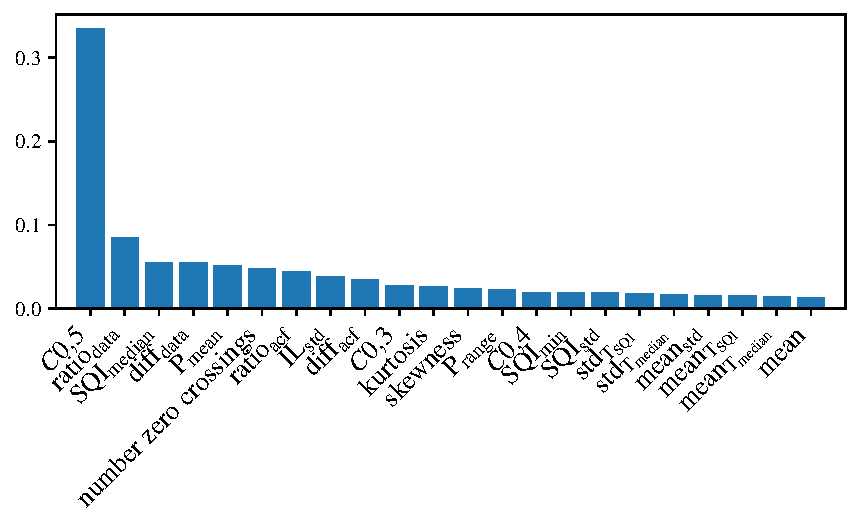
\includegraphics[width=\textwidth]{pic/xgb-clf-final-importances.pdf}
 			\caption{\ac{XGB}-Klassifikator}
 		\end{subfigure}
    	\begin{subfigure}{.49\textwidth}
    		\centering
 			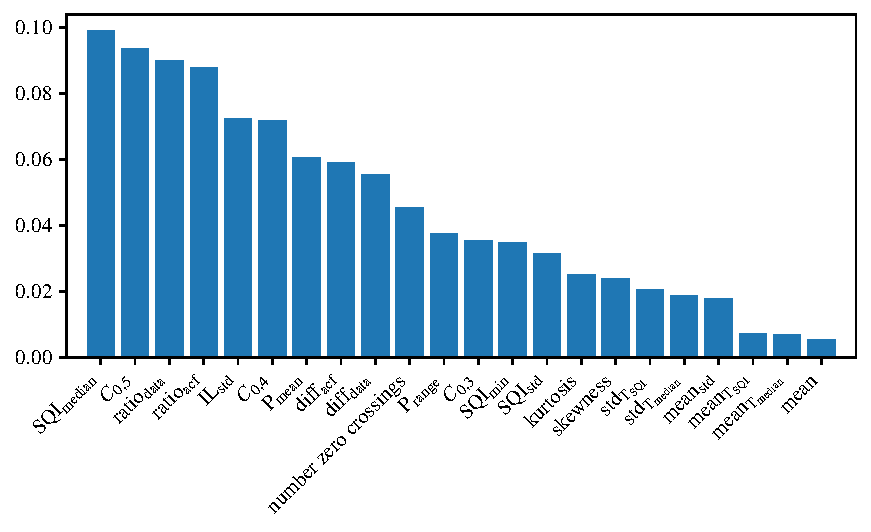
\includegraphics[width=\textwidth]{pic/rf-clf-final-importances.pdf}
 			\caption{\ac{RF}-Klassifikator}
 		\end{subfigure}
 	\caption{Vergleich der Wichtigkeit der Merkmale zwischen \ac{RF}-Klassifikator und \ac{XGB}-Klassifikator}
 	\label{fig:importances-comparison-rf-xgb-clf}
 \end{figure}

Bei der Betrachtung der Regressionsmodelle zeigt sich, dass es bei dem \ac{XGB}-Regressor zwei Merkmale gibt, die bedeutend wichtiger als der Rest sind: Erneut $C_{0,5}$ und $\text{ratio}\textsubscript{data}$. Das \ac{RF}-Modell zeigt auch hier eine gleichmäßigere Verteilung der Wichtigkeit der Merkmale. Die Wichtigkeit der übrigen Merkmale ist, wie in Abbildung \ref{fig:importances-comparison-rf-xgb-regr} zu sehen, teilweise ähnlich verteilt.

 \begin{figure}[h]
 	\centering
		\begin{subfigure}{.49\textwidth}
			\centering
 			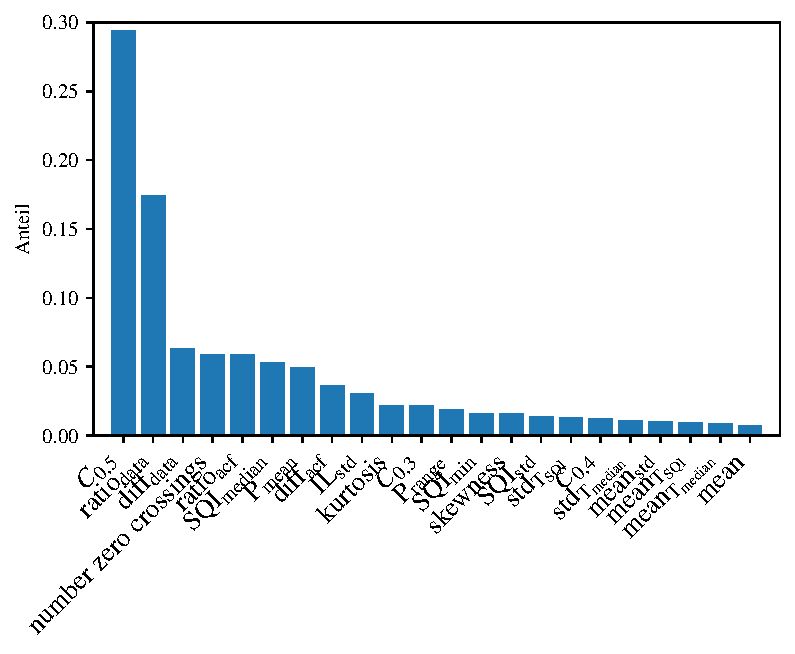
\includegraphics[width=\textwidth]{pic/xgb-regr-final-importances.pdf}
 			\caption{\ac{XGB}-Regressor}
 		\end{subfigure}
    	\begin{subfigure}{.49\textwidth}
    		\centering
 			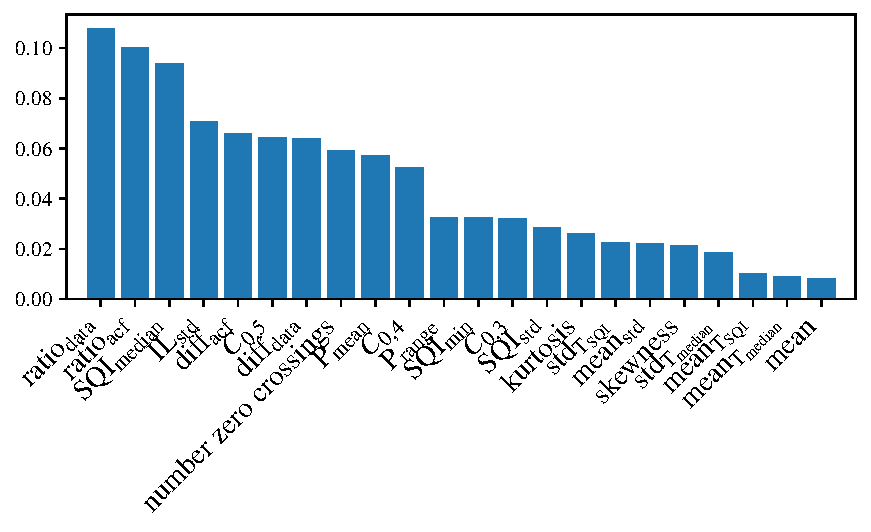
\includegraphics[width=\textwidth]{pic/rf-regr-final-importances.pdf}
 			\caption{\ac{RF}-Regressor}
 		\end{subfigure}
 	\caption{Vergleich der Wichtigkeit der Merkmale zwischen \ac{RF}-Regressor und \ac{XGB}-Regressor}
 	\label{fig:importances-comparison-rf-xgb-regr}
 \end{figure}
 
 Die \ac{RF}-Modelle gewichten die einzelnen Merkmale bei den vorliegenden Daten ähnlicher als die \ac{XGB}-Modelle. Dennoch sind die Ergebnisse der ersten Evaluation ähnlich. Auch ist die Wichtigkeit der Merkmale zwischen den Klassifikations- und Regressionsmodellen ähnlich. Insgesamt zeigen die Regressionsmodelle aber eine überlegende Performance. Eine genauere Evaluation der Coverage und der Verteilung von $E\textsubscript{HR}$ wird für den \ac{RF}-Regressor durchgeführt. Zum Vergleich werden die Ergebnisse der Klassifizierung anhand der Intervallschätzer des \ac{CLIE}-Algorithmus für $q\textsubscript{th}=0{,}3$ und $c\textsubscript{th}$ gezeigt, da mit diesen Schwellwerten ebenfalls eine Reduzierung des \ac{MAE} mit einer vergleichbaren Coverage von 37,87\,\% erreicht wurde. Der Vergleich der erreichten Coverage unter einem bestimmten $E\textsubscript{HR}$, sichtbar in Tabelle \ref{fig:own-coverage-default}, zeigt deutlich, dass die Coverage geringer Fehler deutlich erhöht werden konnte. 
 
  \begin{table}[h]
 	\centering
  	\begin{tabular}{l || c | c | c}
 											& insgesamt 		& \ac{RF}-Regressor & \ac{CLIE}-Intervallschätzer\\\hline
 		$E\textsubscript{HR} < 5$\,\si{FE} 	&  32{,}61\,\% 	& 23,93\,\% 			& 18,32\,\%\\
 		$E\textsubscript{HR} < 10$\,\si{FE} 	&  43{,}21\,\% 	& 28,80\,\% 			& 21,34\,\%\\
 		$E\textsubscript{HR} < 15$\,\si{FE} 	&  51{,}64\,\% 	& 32,17\,\% 			& 23,35\,\%\\
 		$E\textsubscript{HR} < 20$\,\si{FE} 	&  59{,}38\,\% 	& 35,03\,\% 			& 25,12\,\%\\
 	\end{tabular}
 	\caption[Coverage unter bestimmten Fehlern $E\textsubscript{HR}$ nach Klassifikation mittels \ac{RF}-Regressor]{Coverage unter bestimmten Fehlern $E\textsubscript{HR}$ nach Klassifikation mittels \ac{RF}-Regressor}
 	\label{fig:own-coverage-default}
 \end{table}
 
 Auch eine Untersuchung der Verteilung von $E\textsubscript{HR}$ auf den als informativ klassifizierten Segmenten zeigt im Verglich, dass der Anteil des Signals mit einem Fehler $E\textsubscript{HR} > 20\,\si{FE}$ stark gesenkt werden konnte. Auch liegt der durchschnittliche \ac{MAE} der falsch-negativen Segmente bei 4,36\,\si{FE}, was über dem Durchschnitt aller als informativ klassifizierten Segmente von 3,28\,\si{FE} liegt.
 
 \begin{figure}[h]
 	\centering
		\begin{subfigure}{.45\textwidth}
			\centering
 			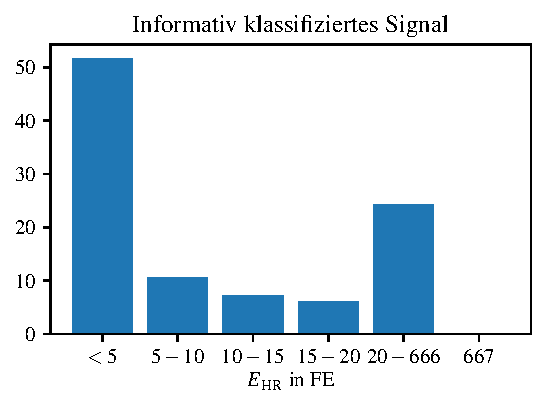
\includegraphics[scale=0.7]{pic/rf-own-final-10-positives.pdf}
 			\caption{\ac{RF}-Regressor}
 		\end{subfigure}
    	\begin{subfigure}{.45\textwidth}
    		\centering
 			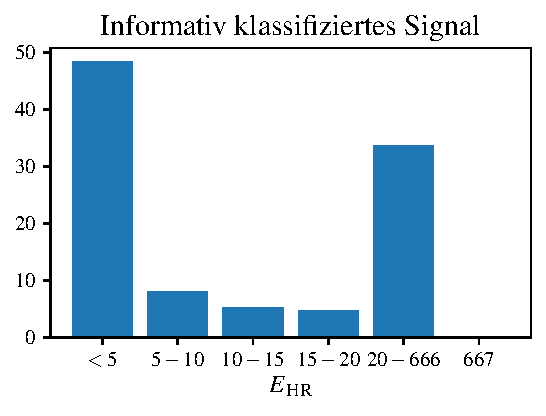
\includegraphics[scale=0.7]{pic/brueser03-positives.pdf}
 			\caption{Ähnlichkeit der Intervallschätzer}
 		\end{subfigure}
 	\caption{Verteilung von $E\textsubscript{HR}$ bei den als informativ klassifizierten Segmenten}
 	\label{fig:own-10-positives}
 \end{figure}
 
 Mit den im Rahmen dieser Arbeit entwickelten Modellen kann also die Signalqualität zuverlässiger als bisher beurteilt werden. Die Coverage durch die Klassifikation konnte erhöht und der \ac{MAE} der als informativ klassifizierten Segmente gesenkt werden.

\section{Einfluss des Schwellwertes der Annotation}

Nachdem die generelle Performance der Modelle untersucht wurde, wird nun der Einfluss des verwendeten Schwellwertes $E\textsubscript{th}$ der Annotation untersucht. Dafür werden die vier Modelle jeweils für vier Schwellwerte $E\textsubscript{th}$ trainiert: $E\textsubscript{th} \in \{5, 10, 15, 20\}$.

Die Ergebnisse der Klassifikationsmodelle sind in Tabelle \ref{fig:var-eth-clf} gezeigt. Für diese Modelle ergibt sich für niedrigere Schwellwerte $E\textsubscript{th}$ jeweils eine niedrigere Coverage und ein niedrigerer \ac{MAE}. Die Variation des \ac{MAE} beträgt zwischen $E\textsubscript{th}= 5\,\si{FE}$ und $E\textsubscript{th} = 20\,\si{FE}$ allerdings nur gut 2\,\si{FE} beim \ac{RF}-Klassifikator bzw. 2,5\,\si{FE} beim \ac{XGB}-Klassifikator. Die Coverage kann dabei um ca. 15\,\% für das \ac{RF}-Modell und um ca. 18\,\% für das \ac{XGB}-Modell erhöht werden. Wie wichtig die Genauigkeit der Herzratenschätzung im Vergleich zur Coverage ist, hängt vom Anwendungsfall ab, allerdings ist der Gewinn durch die deutlich erhöhte Coverage vermutlich in den meisten Fällen größer. Für alle Schwellwerte ist weiterhin eine Trennung der beiden Klassen möglich, wobei jeweils die Modelle mit $E\textsubscript{th}= 5\text{\,}\si{FE}$ die beste Trennung ermöglichen. Es kann also auch sinnvoll sein, lediglich den Schwellwert des Klassifikationsmodells anzupassen. Eine genauere Untersuchung der Auswirkungen durch eine solche Variation ist im Rahmen dieser Arbeit allerdings nicht möglich. In diesen Untersuchungen zeigt sich ebenfalls, dass der \ac{XGB}-Klassifikator tendenziell eine höhere Coverage mit höherem \ac{MAE} erreicht als das \ac{RF}-Modell.

\begin{table}[H]
	\begin{subfigure}{\textwidth}
	\centering
	\begin{tabular}{l || c | c | c | c | c}
								& insgesamt	& $E\textsubscript{th}=5$	& $E\textsubscript{th}=10$	& $E\textsubscript{th}=15$	& $E\textsubscript{th}=20$	\\ \hline
	Coverage annotiert [\%]		& -			& 32,61						& 43{,}21 					& 51,64						& 59,45\\
 	Coverage klassifiziert [\%]	& -			& 29,30						& 34,90 					& 42,46						& 53,78\\
 	\ac{MAE} [FE]				& 21{,}85	& 11,39						& 11,86						& 12,44						& 13,27\\
 	F1-Score 					& -			& 0,59						& 0,60						& 0,64						& 0,70\\
 	AUC 						& -			& 0,78						& 0,75						& 0,73						& 0,73\\
 	\end{tabular}	
	\caption{\ac{RF}-Klassifikator}
	\end{subfigure}
	\begin{subfigure}{\textwidth}
	\centering
	\begin{tabular}{l || c | c | c | c | c}
	\multicolumn{6}{l}{	}	\\
								& insgesamt	& $E\textsubscript{th}=5$	& $E\textsubscript{th}=10$	& $E\textsubscript{th}=15$	& $E\textsubscript{th}=20$	\\ \hline
	Coverage annotiert [\%]		& -			& 32,61						& 43{,}21 					& 51,64						& 59,45\\
 	Coverage klassifiziert [\%]	& -			& 31,51						& 41,99 					& 51,15						& 59,73\\
 	\ac{MAE} [FE]				& 21{,}85	& 11,39						& 12,44						& 13,23						& 13,86\\
 	F1-Score 					& -			& 0,59						& 0,63						& 0,67						& 0,73\\
 	AUC 						& -			& 0,77						& 0,75						& 0,73						& 0,73\\
 	\end{tabular}	
	\caption{\ac{XGB}-Klassifikator}
	\end{subfigure}
	\caption{Variation des Schwellwerts $E\textsubscript{th}$ der Annotation bei den Klassifikationsmodellen}
	\label{fig:var-eth-clf}
\end{table}

Betrachtet man die Coverage unter bestimmten Fehlern für $E\textsubscript{th}= 5\text{\,}\si{FE}$ und $E\textsubscript{th}= 20\text{\,}\si{FE}$ im Vergleich, wird deutlich, dass durch eine Erhöhung von $E\textsubscript{th}$ in der Annotation auch Segmente mit niedrigem Fehler deutlich zuverlässiger miterfasst werden. Der direkte Vergleich ist in Tabelle \ref{fig:xgb-clf-cov-eth} für den \ac{XGB}-Klassifikator gezeigt.

\begin{table}[H]
	\centering
  	\begin{tabular}{l || c | c | c}
 											& insgesamt 		& $E\textsubscript{th}= 5\text{\,}\si{FE}$ & $E\textsubscript{th}= 20\text{\,}\si{FE}$\\\hline
 		$E\textsubscript{HR} < 5$\,\si{FE} 	&  32{,}61\,\% 	& 18,85\,\% 			& 26,06\,\%\\
 		$E\textsubscript{HR} < 10$\,\si{FE} 	&  43{,}21\,\% 	& 21,70\,\% 			& 33,22\,\%\\
 		$E\textsubscript{HR} < 15$\,\si{FE} 	&  51{,}64\,\% 	& 23,33\,\% 			& 38,65\,\%\\
 		$E\textsubscript{HR} < 20$\,\si{FE} 	&  59{,}38\,\% 	& 24,65\,\% 			& 43,35\,\%\\
 	\end{tabular}
 	\caption{Coverage unter bestimmten Fehlern $E\textsubscript{HR}$ nach Klassifikation mittels \ac{XGB}-Klassifikator für verschiedene Schwellwerte der Annotation}
 	\label{fig:xgb-clf-cov-eth}
\end{table}

Bei den Regressionsmodellen ist der Einfluss der Variation von $E\textsubscript{th}$ deutlich stärker, wie in Tabelle\,\ref{fig:var-eth-regr} zu sehen ist. Hier variiert der \ac{MAE} um ca. 5,5\,\si{FE} für das \ac{RF}-Modell und um ca. 4,5\,\si{FE} für den \ac{XGB}-Regressor. Die Coverage zeigt eine stärkere Variation von knapp 60\,\% bzw. für das \ac{XGB}-Modell knapp 50\,\%. Auch sind die erreichten durchschnittlichen Fehler für $E\textsubscript{th}= 20\text{\,}\si{FE}$ 1 bis 2\,\si{FE} höher als bei den Klassifikationsmodellen und für $E\textsubscript{th}= 5\text{\,}\si{FE}$ jeweils 1 bis 2\,\si{FE} niedriger. Die \ac{AUC} dagegen verhält sich relativ ähnlich zu den Klassifikationsmodellen.

\begin{table}[H]
	\begin{subfigure}{\textwidth}
	\centering
	\begin{tabular}{l || c | c | c | c | c}
								& insgesamt	& $E\textsubscript{th}=5$	& $E\textsubscript{th}=10$	& $E\textsubscript{th}=15$	& $E\textsubscript{th}=20$	\\ \hline
	Coverage annotiert [\%]		& -			& 32,61						& 43{,}21 					& 51,64						& 59,45\\
 	Coverage klassifiziert [\%]	& -			& 20,19						& 46,36 					& 71,16						& 79,47\\
 	\ac{MAE} [FE]				& 21{,}85	& 9,83						& 12,57						& 14,61						& 15,39\\
 	F1-Score 					& -			& 0,52						& 0,64						& 0,72						& 0,78\\
 	AUC 						& -			& 0,77						& 0,75						& 0,74						& 0,73\\
 	\end{tabular}	
	\caption{\ac{RF}-Regressor}
	\end{subfigure}
 	\begin{subfigure}{\textwidth}
	\centering
	\begin{tabular}{l || c | c | c | c | c}
	\multicolumn{6}{l}{	}	\\
								& insgesamt	& $E\textsubscript{th}=5$	& $E\textsubscript{th}=10$	& $E\textsubscript{th}=15$	& $E\textsubscript{th}=20$	\\ \hline
	Coverage annotiert [\%]		& -			& 32,61						& 43{,}21 					& 51,64						& 59,45\\
 	Coverage klassifiziert [\%]	& -			& 26,76						& 47,59 					& 63,74						& 74,18\\
 	\ac{MAE} [FE]				& 21{,}85	& 10,52						& 12,66						& 14,04						& 14,94\\
 	F1-Score 					& -			& 0,55						& 0,64						& 0,71						& 0,77\\
 	AUC 						& -			& 0,75						& 0,74						& 0,73						& 0,73\\
 	\end{tabular}	
	\caption{\ac{XGB}-Regressor}
	\end{subfigure}
	\caption{Variation des Schwellwerts $E\textsubscript{th}$ der Annotation bei den Regressionsmodellen}
	\label{fig:var-eth-regr}
\end{table}

Auch hier wird die Coverage unter bestimmten Fehlern $E\textsubscript{HR}$ untersucht. Die Ergebnisse der Regressionsmodell für niedrige $E\textsubscript{th}$ weisen eine deutlich geringere Coverage auf, aber für $E\textsubscript{th} = 20$ wird nahezu alles informative Signal erkannt. Vor allem fällt auf, dass bei $E\textsubscript{th}= 5\text{\,}\si{FE}$ sehr viel Signal mit nur geringem Fehler nicht erkannt wird. Der Vergleich zwischen $E\textsubscript{th}= 5\text{\,}\si{FE}$ und $E\textsubscript{th}= 5\text{\,}\si{FE}$ beim \ac{RF}-Regressor ist in Tabelle\,\ref{fig:rf-regr-cov-eth} gezeigt.

\begin{table}[H]
	\centering
  	\begin{tabular}{l || c | c | c}
 											& insgesamt 		& $E\textsubscript{th}= 5\text{\,}\si{FE}$ & $E\textsubscript{th}= 20\text{\,}\si{FE}$\\\hline
 		$E\textsubscript{HR} < 5$\,\si{FE} 	&  32{,}61\,\% 	& 13,75\,\% 			& 31,14\,\%\\
 		$E\textsubscript{HR} < 10$\,\si{FE} 	&  43{,}21\,\% 	& 15,05\,\% 			& 40,48\,\%\\
 		$E\textsubscript{HR} < 15$\,\si{FE} 	&  51{,}64\,\% 	& 15,75\,\% 			& 47,78\,\%\\
 		$E\textsubscript{HR} < 20$\,\si{FE} 	&  59{,}38\,\% 	& 16,36\,\% 			& 54,37\,\%\\
 	\end{tabular}
 	\caption{Coverage unter bestimmten Fehlern $E\textsubscript{HR}$ nach Klassifikation mittels \ac{RF}-Regressor für verschiedene Schwellwerte der Annotation}
 	\label{fig:rf-regr-cov-eth}
\end{table}

Die Untersuchungen zeigen, dass die Wahl von $E\textsubscript{th}$ einen großen Einfluss vor allem auf die erreichte Coverage der Klassifizierung hast. Auch hier muss abgewogen werden, ob hohe Genauigkeit oder hohe Coverage wichtiger sind, allerdings ist der Gewinn der Coverage durch die Wahl eines höheren Schwellwertes $E\textsubscript{th}$ in den meisten Fällen vermutlich größer.

\section{Einfluss der Segmentlänge}

Neben dem Einfluss des Schwellwertes der Annotation $E\textsubscript{th}$ wird auch der Einfluss der verwendeten Segmentlänge $s$ untersucht. Für diese Untersuchung wird aufgrund der Ergebnisse der vorherigen Untersuchungen $E\textsubscript{th}=20$ gewählt. Untersuchte Segmentlänge sind 5, 10, 20 und 30 Sekunden.

Bei den Klassifikationsmodellen zeigt sich deutlich, dass mit steigender Segmentlänge die Coverage höher und der \ac{MAE} niedriger wird, siehe Tabelle\,\ref{fig:var-s-clf}. Es muss zusätzlich beachtet werden, dass der \ac{MAE} über die Segmente insgesamt mit steigender Segmentlänge ebenfalls sinkt, die Verbesserung also eventuell darin begründet ist. Auch der F1-Score steigt mit der Segmentlänge; die \ac{AUC} dagegen wird etwas niedriger. Bei dem \ac{RF}-Modell sind die Veränderungen in \ac{MAE} und Coverage etwas größer als bei dem \ac{XGB}-Klassifikator. Alles in allem führen größere Segmente bei den Klassifikationsmodellen zu besseren Ergebnissen bezüglich Coverage und \ac{MAE}, allerdings lassen sich die beiden Klassen etwas schlechter voneinander trennen. 

\begin{table}[H]
	\begin{subfigure}{\textwidth}
	\centering
	\begin{tabular}{l || c | c | c | c }
								& $s = 5$	& $s=10$		& $s=20$		& $s=30$	\\ \hline
	Coverage annotiert [\%]		& 39,30		& 43,21	 	& 45,47		& 45,87\\
	\ac{MAE} insgesamt [FE]		& 25,96		& 21,85		& 19,99		& 19,31\\\hline
 	Coverage klassifiziert [\%]	& 45,94		& 53,78 		& 60,93		& 62,01\\
 	\ac{MAE} klassifiziert [FE]	& 14,20		& 13,27		& 13,03		& 12,68\\
 	F1-Score 					& 0,62		& 0,65		& 0,66		& 0,67\\
 	AUC 						& 0,75		& 0,74		& 0,73		& 0,73\\
 	\end{tabular}	
	\caption{\ac{RF}-Klassifikator}
	\end{subfigure}
	\begin{subfigure}{\textwidth}
	\centering
	\begin{tabular}{l || c | c | c | c }
	\multicolumn{5}{l}{	}	\\
								& $s = 5$	& $s=10$		& $s=20$		& $s=30$	\\ \hline
								
	Coverage annotiert [\%]		& 39,30		& 43,21	 	& 45,47		& 45,87\\
	\ac{MAE} insgesamt [FE]		& 25,96		& 21,85		& 19,99		& 19,31\\\hline
 	Coverage klassifiziert [\%]	& 54,18		& 59,73 		& 64,81		& 67,00\\
 	\ac{MAE} klassifiziert [FE]	& 14,20		& 13,86		& 13,23		& 13,12\\
 	F1-Score 					& 0,61		& 0,65		& 0,66		& 0,67\\
 	AUC 						& 0,73		& 0,73		& 0,72		& 0,72\\
 	\end{tabular}		
	\caption{\ac{XGB}-Klassifikator}
	\end{subfigure}
	\caption{Variation des Segmentlänge $s$ bei den Klassifikationsmodellen}
	\label{fig:var-s-clf}
\end{table}

Betrachtet man die Coverage aufgeschlüsselt nach bestimmten Fehlern $E\textsubscript{HR}$, zeigt sich, dass der Fehler wie schon beschrieben bei längeren Segmenten niedriger ist, aber auch, dass die Klassifikation bei längeren Segmenten näher an der Annotation ist. Für den \ac{RF}-Klassifikator ist die Coverage für die Segmentlängen $s=5$ und $s=30$ in Tabelle\,\ref{fig:rf-clf-cov-s} aufgeschlüsselt.

\begin{table}[H]
	\centering
  	\begin{tabular}{l || c | c || c | c}
  											& \multicolumn{2}{c ||}{$s=5$}	& \multicolumn{2}{c}{$s=30$}\\
 											& insgesamt 		& klassifiziert & insgesamt		& klassifiziert\\\hline
 		$E\textsubscript{HR} < 5$\,\si{FE} 	&  29,88\,\% 	& 21,72\,\% 		& 33,33\,\%		& 27,45\,\%\\
 		$E\textsubscript{HR} < 10$\,\si{FE} 	&  39,29\,\% 	& 26,36\,\% 		& 45,86\,\%		& 36,16\,\%\\
 		$E\textsubscript{HR} < 15$\,\si{FE} 	&  47,38\,\% 	& 30,07\,\% 		& 54,97\,\%		& 42,23\,\%\\
 		$E\textsubscript{HR} < 20$\,\si{FE} 	&  55,17\,\% 	& 33,48\,\% 		& 62,85\,\%		& 47,11\,\%\\
 	\end{tabular}
 	\caption{Coverage unter bestimmten Fehlern $E\textsubscript{HR}$ nach Klassifikation mittels \ac{RF}-Klassifikator für verschiedene Segmentlängen s}
 	\label{fig:rf-clf-cov-s}
\end{table}

Bei den Regressionsmodellen ist, wie in Tabelle\,\ref{fig:var-s-regr} gezeigt, ähnliches zu beobachten. Hier ist der Effekt auf den \ac{MAE} etwas stärker als bei den Klassifikationsmodellen; bei beiden Modellen beträgt die Veränderung über 2\,\si{FE}. Auch hier ist er beim \ac{RF}-Modell etwas stärker. Die Veränderung der Coverage ist beim \ac{RF}-Regressor dagegen nur minimal; zwischen $s=5$ und $s=30$ beträgt der Unterschied nur knapp 1,5\,\%. Auch beim \ac{XGB}-Modell ist die Veränderung der Coverage weniger stark, als bei den Klassifikationsmodellen, aber zumindest bei ca. 8\,\%.


\begin{table}[H]
	\begin{subfigure}{\textwidth}
	\centering
	\begin{tabular}{l || c | c | c | c }
								& $s = 5$	& $s=10$		& $s=20$		& $s=30$	\\ \hline
	Coverage annotiert [\%]		& 39,30		& 43,21	 	& 45,47		& 45,87\\
	\ac{MAE} insgesamt [FE]		& 25,96		& 21,85		& 19,99		& 19,31\\\hline
 	Coverage klassifiziert [\%]	& 78,93		& 79,47 		& 80,15		& 80,31\\
 	\ac{MAE} klassifiziert [FE]	& 17,62		& 15,39		& 14,35		& 14,01\\
 	F1-Score 					& 0,62		& 0,66		& 0,68		& 0,68\\
 	AUC 						& 0,76		& 0,75		& 0,74		& 0,73\\
 	\end{tabular}		
	\caption{\ac{RF}-Regressor}
	\end{subfigure}
	\begin{subfigure}{\textwidth}
	\centering
	\begin{tabular}{l || c | c | c | c } %TODO
	\multicolumn{5}{l}{	}	\\
								& $s = 5$	& $s=10$		& $s=20$		& $s=30$	\\ \hline
	Coverage annotiert [\%]		& 39,30		& 43,21	 	& 45,47		& 45,87\\
	\ac{MAE} insgesamt [FE]		& 25,96		& 21,85		& 19,99		& 19,31\\\hline
 	Coverage klassifiziert [\%]	& 69,40		& 74,18 		& 76,69		& 77,14\\
 	\ac{MAE} klassifiziert [FE]	& 16,34		& 14,94		& 14,17		& 13,96\\
 	F1-Score 					& 0,63		& 0,66		& 0,68		& 0,68\\
 	AUC 						& 0,74		& 0,74		& 0,72		& 0,71\\
 	\end{tabular}
	\caption{\ac{XGB}-Regressor}
	\end{subfigure}
	\caption{Variation des Segmentlänge $s$ bei den Regressionsmodellen}
	\label{fig:var-s-regr}
\end{table}

Der direkte Vergleich der Verteilung von $E\textsubscript{HR}$ auf den als informativ klassifizierten Segmenten zeigt deutlich, dass bei $s=30$ ein deutlich größerer Teil des als informativ klassifizierten Signals einen kleinen Fehler $E\textsubscript{HR}$ aufweist. Bei $s=5$ dagegen ist der Anteil des Signals mit $E\textsubscript{HR} > 20$ ähnlich groß wie der mit $E\textsubscript{HR} < 5$.

 \begin{figure}[H]
 	\centering
		\begin{subfigure}{.45\textwidth}
			\centering
 			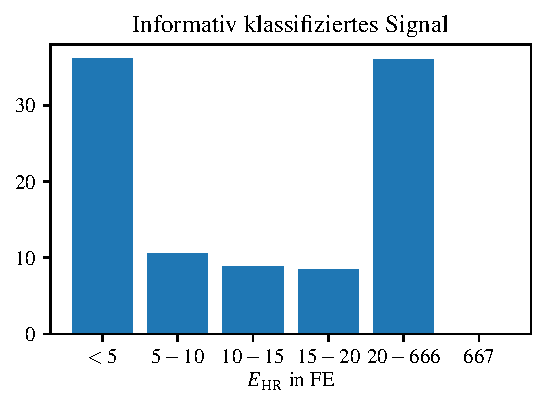
\includegraphics[scale=0.7]{pic/rf-regr-s5-h20-positives.pdf}
 			\caption{$s=5$}
 		\end{subfigure}
    	\begin{subfigure}{.45\textwidth}
    		\centering
 			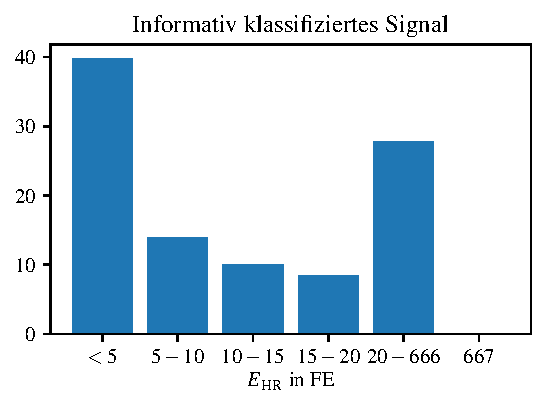
\includegraphics[scale=0.7]{pic/rf-regr-s30-h20-positives.pdf}
 			\caption{$s=30$}
 		\end{subfigure}
 	\caption{Verteilung von $E\textsubscript{HR}$ bei den vom \ac{RF}-Regressor als informativ klassifizierten Segmenten mit verschiedenen Segmentlängen $s$}
 	\label{fig:rf-regr-var-s-positives}
 \end{figure}

 Bei der Bewertung muss jedoch auch beachtet werden, dass die Herzrate über die Berechnung des Medians der geschätzten Intervalllängen wird, also dementsprechend mit steigender Segmentlänge auch robuster wird. Auch hier gilt aus diesem Grund, dass die Wahl der Segmentlänge von dem Anwendungsfall abhängt, tendenziell aber längere Segmente zu besseren Ergebnissen führen.



